\documentclass[preprint]{aastex} 

\usepackage[top=1in, bottom=1in, left=1in, right=1in]{geometry}
\usepackage{amsmath}
\usepackage{graphicx}
\usepackage{mdwlist}
\usepackage{natbib}
\usepackage{natbibspacing}
\setlength{\bibspacing}{0pt}
\setlength{\parskip}{0pt}
\setlength{\parsep}{0pt}
\setlength{\headsep}{0pt}  
\setlength{\topskip}{0pt}
\setlength{\topmargin}{0pt}
\setlength{\topsep}{0pt}
\setlength{\partopsep}{0pt}
\setlength{\footnotesep}{8pt}
\pagestyle{empty}
\citestyle{aa}

\newcommand{\simgt}{\stackrel{>}{_{\sim}}}
\def\kperp{k_{\bot}}
\def\kpar{k_{\|}}
\def\k{{\bf k}}
\def\sky{{\theta}}
\def\HI{{H{\small I }}}
\def\HII{{H{\small II }}}
\def\xHI{{x_{\rm\HI}}}

%\usepackage{subfig}
%\usepackage[countmax]{subfloat}

\begin{document}
\title{Project Management Plan}

%A Project Management Plan should be submitted as a supplementary document, and may be up to 
%15 pages in length, although many programs will not need this much space. (Note that the solicitation 
%stated that the management plan should be provided in the Project Description; here we move it to its 
%own supplementary document so that it may be explicitly evaluated by reviewers.)  This section must 
%present a clear and thorough discussion of the project management structure and techniques that will 
%be applied. It may include, for example, a construction plan and schedule, a collaboration management 
%plan, a plan for managing telescope access, or any other pertinent management information. The 
%management plan should identify risks and describe their planned mitigation. If your proposed project 
%would have contributions from sources other than NSF, this section should clearly state both the total 
%cost, and the amount being requested from NSF.  

\section{Collaboration and Governance}
HERA builds upon the organization, tools and linkages developed within the PAPER and MWA collaborations.
In addition to the funded collaborators in the {\em List of Partner Institutions},
HERA includes key partners in South Africa and the UK and is finalizing the collaboration with ASIAA.
\begin{table}[h]
\begin{tabular}{| p{.35\textwidth} | p{.6\textwidth} |}\hline
\textbf{Institution (location)} & \textbf{Role} \\ \hline
SKA-SA (Cape Town, SA) & Partner in site development, logistics, support, science \\ \hline
University KwaZulu Natal (Durban, SA) & Partner in science and support \\ \hline
Cavendish Laboratory (Cambridge, UK) & Partner in development etc \\ \hline
Academia Sinica Institute for Astronomy and Astrophysics (Taipei, Taiwan) & Science, development \\ \hline
\end{tabular}
\label{tab:otherpartners}
\end{table}

\begin{figure}[h]
\centering
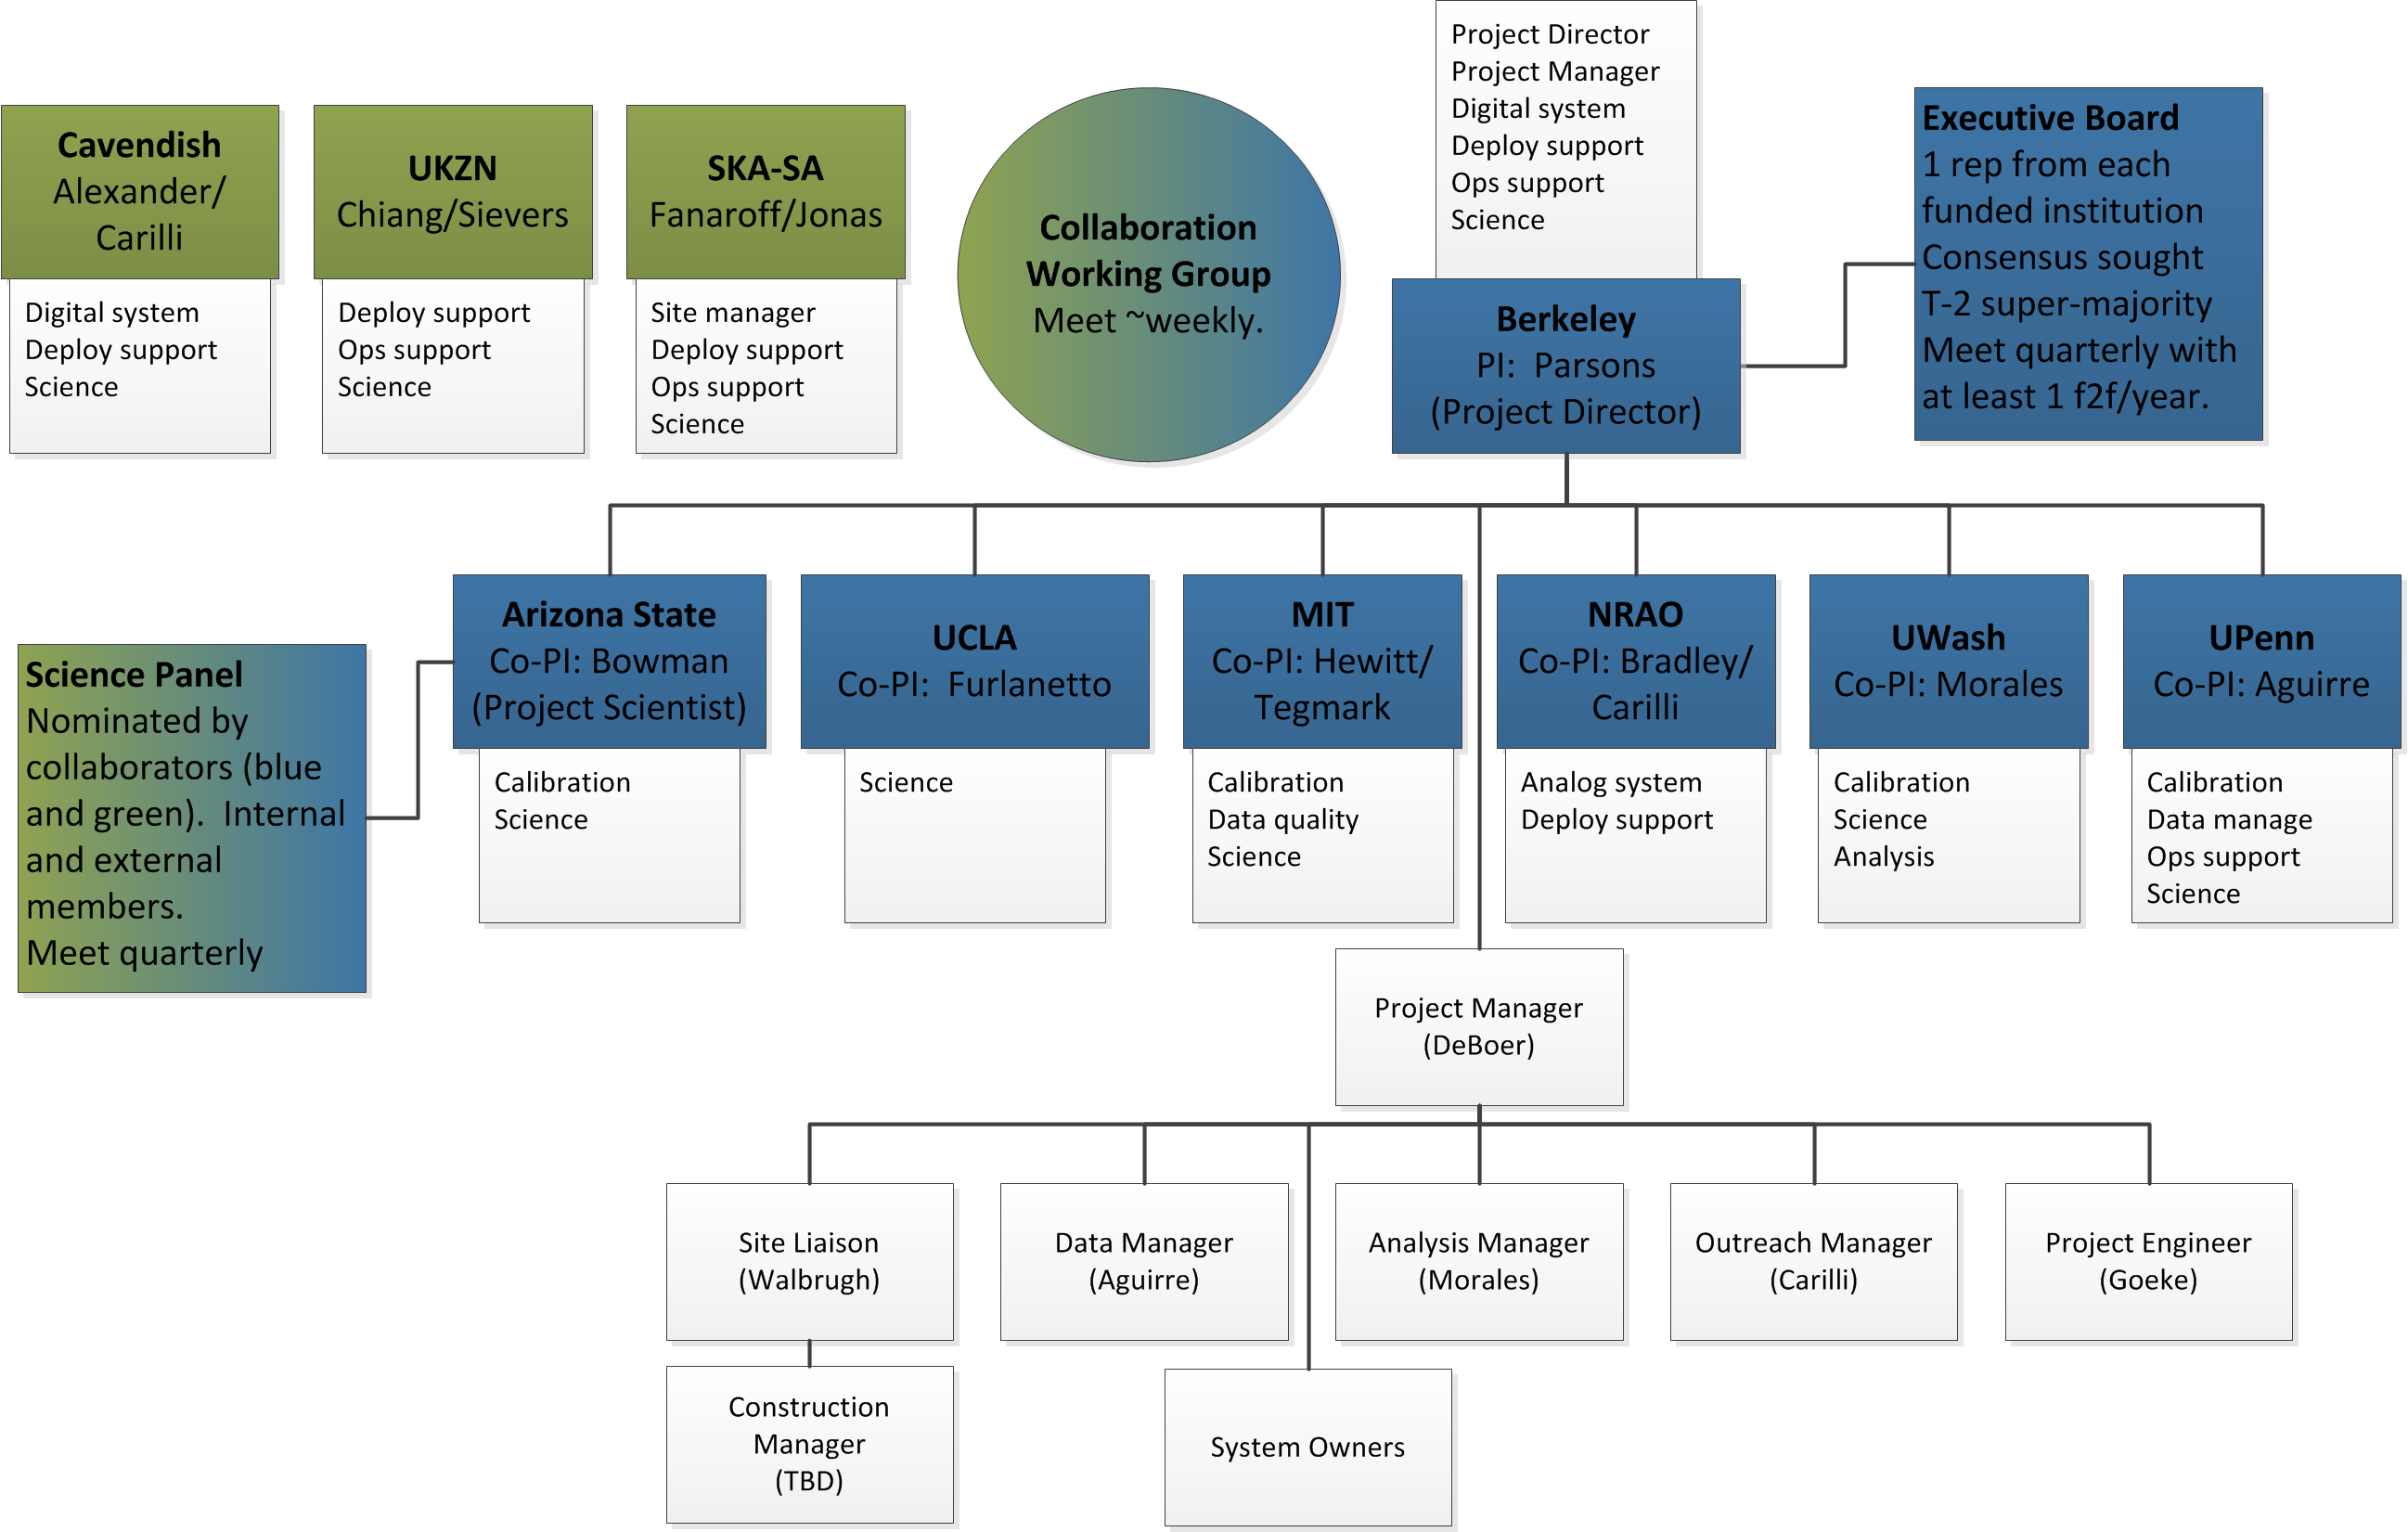
\includegraphics[width=\textwidth]{plots/org.png}
\label{fig:org}
\caption{Org chart showing the collaboration, governance and management.}
\end{figure}

Figure \ref{fig:org} shows the partners and governance. The Executive Board is the
governing board under this proposal and has authority over the science requirements
and the scope of the science goals. It consists of one voting representative from
each of the funded partners, which typically will be the senior scientific partner at
the institution. The Board is Chaired by the Project Director. Though generally
operating on concensus, if matters come to a vote a ``T-2''\footnote{T-2 means that 2
or more must vote against to defeat a motion.} supermajority will be required. The
Executive Board will meet at least quarterly, with at least one face-to-face meeting
per year. The Board is responsible for producing the NSF annual report.

***Other partners are providing funds - membership on EB?  Observers?

A Science Panel, Chaired by the Project Scientist or designate, will meet at least
quarterly to provide advice on the science (scope, progress, support, ). The
composition is determined by the Executive Board, and membership is open to anybody
the Board deems advisable and is willing to serve. Under the auspices of the Science
Panel, one face-to-face workshop will be held per year, rotating its location among
the partners.

The Collaboration Working Group is comprises individuals named by the partner
institutions and will meet approximately weekly to review the project. It is Chaired
by the Project Director or designate and will discuss any and all relevant aspects of
the project. It represents the primary method of frequent communication between the
partners.

\subsection{Communication}
Meetings (telecon Blue Jeans/Webex)  workshop, common repositories, web-site, wiki, email

US-SA

\subsection{Publication}


\section{Management}
Figure \ref{fig:org} also shows the management structure. A project manager has
overall responsibility for planning and tracking to achieve the agreed upon
milestones and budget. The project manager will brief the Executive Board at each
meeting to summarize the state of the project.

The project comprises Components, which are the physical deliverables, and Systems,
which are logical groupings to achieve a function. Systems may be hardware, software
or both. Systems need not be disjoint collections of components. Each System has an
Owner, who is responsible for the System meeting its specifications. The project
manager serves as the Owner of the hardware Components, working with the System
Owners to meet functional specifications.

oversight, tools (RSD, ICD, WBS, Trace), common repo, meetings, owners, change control, wiki

\section{Construction}
plan, schedule, contract summary, milestone summary

\section{Analysis Management}

\section{Budget Overview}

\section{Risk}

\end{document}
